
\subsection{Component Integration Sequence}

In this section, it will be described the integration order of the components of the Application Server.
As notation, an arc $C_1 \rightarrow C_2$ means that the component $C_1$ needs the successful integration of component $C_2$.


\paragraph*{Data Access\\}
The first elements to be integrated are \emph{DBMS}, \emph{Account Data Manager} and \emph{Appointment Data Manager}. 
The integration process starts from this point because other components relies on \emph{Account Data Manager} and \emph{Appointment Data Manager} to store data and retrieves data for computation and visualization.
\begin{figure}[H]
	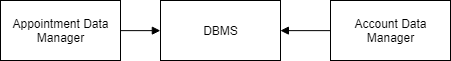
\includegraphics[width=\textwidth, keepaspectratio=true]{Img/FirstStep}
\end{figure}

\paragraph*{Basic Appointment Manager\\}
As second step, \emph{Appointment Data Manager} and \emph{Path Calculator} are integrated in \emph{Appointment Manager}.\\
In this way, it is possible to test how appointments are generated, how are stored and how an appointment interacts with others previous stored appointments.\\
In this step of the integration process, the \emph{Path Calculator} does not consider information about the user preferences, weather conditions or possible strikes, it just provides a path from the departure location to the appointment location.

\begin{figure}[H]
	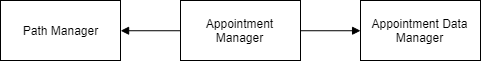
\includegraphics[width=\textwidth, keepaspectratio=true]{Img/SecondStep}
\end{figure}


\paragraph*{Integration of additional info\\}
As third step, \emph{Weather Info Manager}, \emph{Road Info Manager} and \emph{Account Data Manager} are integrated in \emph{Additional Info Façade}.

\begin{figure}[H]
	\centering
	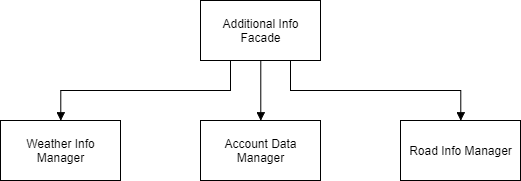
\includegraphics[width=\textwidth, keepaspectratio=true]{Img/ThirdStep}
\end{figure}

\paragraph*{Complete Appointment Manager\\}
As fourth step, the Additional Info Façade is integrated in the Path Calculator component.

\begin{figure}[H]
	\centering
	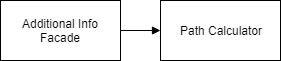
\includegraphics{Img/FourthStep}
\end{figure}

\paragraph*{User Info Management\\}
As final step, it is tested the integration of \emph{Authentication Manager} and \emph{Profile Manager} with \emph{Account Data Manager}.

\begin{figure}[H]
	\centering
	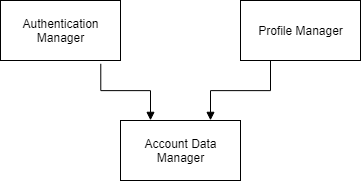
\includegraphics[scale=0.8]{Img/FifthStep}
\end{figure}

\paragraph*{Complete Integration Sequence}
In this diagram is possible to see all the integration steps, numbers on the arrows indicates the precedence, same number on multiple arrows means that is possible to perform the test integration simultaneously.

\begin{figure}[h]
	\centering
	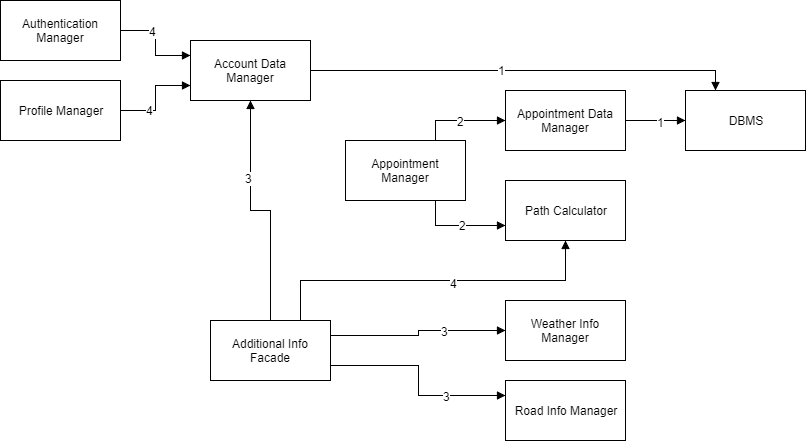
\includegraphics[width=\textwidth, keepaspectratio=true]{Img/IntegrationSequence}
\end{figure}